%!TEX root = Report.tex
\chapter{Introduction}\label{sec:introduction}

In turbomachines very high temperatures are desired to increase the efficiency of the whole system. However, especially downstream of the combustion chamber, fluid temperature can rise above the melting point of the material used for the blades. Special precautions have to be applied as for example coating, thin film cooling and convective cooling. This experiment focusses on internal convective cooling and tries to determine the heat transfer coefficient $\alpha$ by using thermocromic liquid crystals (TLC). Since it remains difficult and costly to measure $\alpha$ inside a turbine blade a ducting channel as an experimental model with comparable non-dimensional characteristic numbers is used. Although the setup allows to determine heat coefficients in sections with different obstacles, this experiment will only focus on v-shaped obstacles causing a turbulent flow.
\begin{figure}[H]
\begin{center}
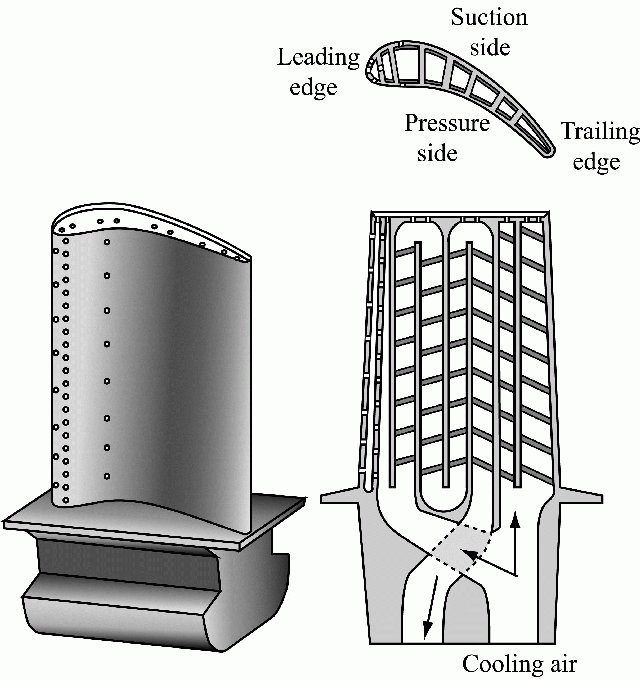
\includegraphics[width=0.6\textwidth]{pics/blade3}
\caption{Internal Cooled Turbine Blade}
\label{pic:blade3}
\end{center}
\end{figure}
